%!TEX root =  main.tex
\newcommand{\one}[1]{\mathbb{I}_{\{#1\}}}s
\newcommand{\Pside}{\P_{\mathrm{side}}\xspace}
\newcommand{\PSAP}{\P_{\mathrm{SAP}}\xspace}
\renewcommand{\P}{\mathcal{P}}

In this section we establish that SAP with strong dominance property is `regret equivalent' to an instance of MAB with side-information and the corresponding algorithm for MAB can be suitably imported to solve SAP efficiently.   

\todoc[inline]{I am thinking that maybe we should skip this general section
and just do the specific reduction as shown below.}
We start with the concept of regret equivalence, which we define for classes of partial monitoring problems.
First, we need some extra notation: Recall that at the end of \cref{sec:background} we agreed that 
a partial monitoring problem can be specified as a 3-tuple $(\A,\Y,\Theta)$ where the elements of $\Theta$ are pairs $(p,r)$,
where for each $a\in \A$ action, $p(\cdot;a)$ is a probability distribution over $\Y$ and $r: \A \to \R$.
Now, let $\Pi(\P)$ denote the set of policies for some partial monitoring problem $\P = (\A,\Y,\Theta)$,
let $\Regret_T(\pi,\theta)$ denote the expected regret of policy $\pi$ on problem instance $\theta\in \Theta$,
and let $\Regret_T^*(\P) = \inf_{\pi\in \Pi(\P)}\sup_{\theta\in \Theta} \Regret_T(\pi,\theta)$ denote the minimax regret on $\P$.

Now let $\P_1 = (\A_1,\Y_1,\Theta_1)$, $\P_1 = (\A_2,\Y_2,\Theta_2)$ be partial monitoring problems.
We say that \emph{$P_1$ is $P_2$-hard}, 
denoted by $P_1 \succeq P_2$, if for any $\pi_1\in \Pi(\P_1)$ policy of $\P_1$ there exists a policy $\pi_2\in \Pi(\P_2)$ of $\P_2$
such that for any $\theta_2\in \Theta_2$ there exists an instance $\theta_1\in \Theta_1$ such that $\Regret_T(\pi_1,\theta_1)\ge \Regret_T(\pi_2,\theta_2)$. An immediate corollary of the definition, justifying the definition, is the following:
\begin{proposition}
If $\P_1\succeq \P_2$ then $\Regret_T^*(\P_1)\ge \Regret_T^*(\Pi_2)$.
\end{proposition}
\begin{proof}
Fix some $\epsilon>0$ and 
let $\pi_1^*\in \Pi(\P_1)$ be an $\epsilon$-minimax-optimal policy of $\P_1$: 
$\sup_{\theta_1\in\Theta_1} \Regret_T(\pi_1^*,\theta_1) \le \Regret_T^*(\P_1)+\epsilon$.
Let $\pi_2^*$ be the policy whose existence follows by the assumption $\P_1\succeq \P_2$.
Let $\theta_2^*\in \Theta_2$ be an instance in $\P_2$ such that 
$\Regret_T(\pi_2^*,\theta_2^*)\ge \sup_{\theta_2\in \Theta_2} \Regret_T(\pi_2^*,\theta_2)-\epsilon$
and let $\theta_1^*\in \Theta_1$ in $\P_1$ whose existence is implied by $\P_1\succeq \P_2$.
Then,
\begin{align*}
 \Regret_T^*(\P_2) &= 
\inf_{\pi_2\in \Pi(\P_2)} \sup_{\theta_2\in \Theta_2} \Regret_T(\pi_2,\theta_2)
\le \sup_{\theta_2\in \Theta_2} \Regret_T(\pi_2^*,\theta_2) 
\le  \Regret_T(\pi_2^*,\theta_2^*)+\epsilon \\
& \le  \Regret_T(\pi_1^*,\theta_1^*)+\epsilon
\le \sup_{\theta_1\in \Theta_1} \Regret_T(\pi_1^*,\theta_1)+\epsilon
\le \Regret_T^*(\P_1) +2\epsilon\,.
\end{align*}
Letting $\epsilon\to 0$ finishes the proof.
\end{proof}
We call two problems \emph{$\P_1,\P_2$ regret-equivalent} if $\P_1$ is $\P_2$-hard and also $\P_2$ is $\P_1$-hard.
It follows immediately that if $\P_1,\P_2$ are regret equivalent then they have the same minimax regret.

A simple way of guaranteeing that a problem $\P_1$ is $\P_2$-hard if we can transform problem instances of $\P_2$ into 
problem instances of $\P_1$ while keeping the reward differences between the action-rewards the same (i.e., allowing the reward to be shifted by a constant).
Formally, we have the following proposition:
\begin{proposition}
Let $\P_i = (\A_i,\Y_i,\Theta_i)$, $i=1,2$ be partial monitoring problems.
Then, $\P_1\succeq \P_2$ holds if there exists $f_{\A}:\A_2\to \A_1$, $f_{\Y}: \Y_2 \to \Y_1$ bijections and $f_{\Theta}:\Theta_2\to \Theta_1$ such that if $(p,r) = f_{\Theta}(p',r')$ for some $(p',r')\in \Theta_2$ then
for any $a',a''\in \A_2$, $y'\in \Y$,
$p'(y';a') = p(f_\Y(y'),f_\A(a'))$ and $r'(a')-r'(a'') = r(f_\A(a')) - r(f_\A(a''))$.
\end{proposition}
\begin{proof}
The proof follows directly from two simple observations 
that hold for any instance $\theta_2 = (p',r')$ of $\P_2$: 
First, if $a_2^*$ is an optimal action for $\theta_2$
then $a_1^*=f_\A(a_2^*)$ is an optimal action for instance $(p,r) = f_\Theta(\theta_2)$.
Second, any policy $\pi_1$ of $\P_1$ can be translated using the maps $f_\A$ and $f_\Y$ into a policy $\pi_2$ of $\P_2$ (regardless of $\theta_2$) such that
for any $t\ge 1$,
$P_{\pi_2,\theta_2,t}$ is the push-forward distribution 
of $P_{\pi_1,\theta_1}$ under $f_t:(\A_2\times \Y_2)^t \to (\A_1\times \Y_1)^t$
defined by $f_t(a_1',y_1',\dots,a_t',y_t') = (f_\A(a_1'),f_\Y(y_1'),\dots,f_\A(a_t'),f_\Y(y_t'))$. 
Here $\pi_2(a'_t|a_1',y_1',\dots,a_t',y_t') = \pi_1( f_\A(a_t')| f_\A(a_1'),f_\Y(y_1'),\dots,f_\A(a_t'),f_\Y(y_t'))$ and recall that $P$ is called the push-forward measure of $Q$ under $f:\mathrm{dom}(Q)\to \mathrm{dom}(P)$ if $P$ is the distribution of $f(X)$ where $X\sim Q$.
Both claims can be seen to hold by a simple direct calculation whose details are left 
to the reader.
From the two claims it follows that $\Regret_T(\pi_1,\theta_1)
= \Regret_T(\pi_2,\theta_2)$, showing that $\P_1$ and $\P_2$ are indeed
regret equivalent.
\end{proof}

\todo[inline]{Here is the actual reduction. Maybe let's just keep this part?}
Let us now show how to reduce SAP under strong dominance to a specific 
bandit with side-observations.
Let $\PSAP$ be the set of SAPs with action set $\A = [K]$.
The corresponding bandit problems will have the same action set,
while for action $k\in [K]$ the neighborhood set is $N(k) = [k]$.
Take any instance $(P,c)\in \PSAP$ and let $(Y,Y^1,\dots,Y^K) \sim P$.
We let the reward distribution for arm $k$ in the corresponding bandit problem
be a shifted Bernoulli distribution.
In particular, the cost of arm $k$ follows the distribution of 
$\one{Y^k\ne Y^1} + (c_1+\dots+c_k)$ (we use costs here to avoid flipping signs).
The costs for different arms are defined to be independent of each other.
Let $\Pside$ denote the set of resulting bandit problems and let $f:\PSAP \to \Pside$
be the map that transforms SAP instances to bandit instances by following the
transformation that was just described.
\todoc[inline]{
Ok, so if they are independent of each other, then the joint distributions will not be 
same as if they were not independent of each other.
Independence may lose information (e.g., may increase variance?).
If we define them not to be independent of each other, we will need to be careful
with the algorithms defined for bandits with side-observation: Do they use
(in their proof) independence of rewards underlying different arms?
I would think that they are not.
The downside of not defining independent rewards is that the specification of
bandits with side observations must allow this -- complicating things a bit in the background.
Another executive decision we should make is whether we like to see both costs and 
rewards.
}
Now let $\pi\in \Pi(\Pside)$ be a policy for $\Pside$.
Policy $\pi$ can also be used on any $(P,c)$ instance in $\PSAP$ in an obvious way:
In particular, given the history of actions and observations $A_1,U_1,\dots,A_t,U_t$
in $\theta=(P,c)$ where $U_s = (Y_s,Y_s^1,\dots,Y_s^{A_s})$ such that 
the distribution of $U_s$ given that $A_s=a$ is $P$ marginalized to $\Y^{a}$,
the next action to be taken is 
$A_{t+1}\sim \pi(\cdot| A_1, V_1,\dots,A_t,V_t)$, where
$V_s = (\one{Y_s^1\ne Y_s^2}+c_1,\dots,\one{Y_s^1\ne Y_s^{A_s}}+c_1+\dots+c_{A_s})$. Let the resulting policy be denoted by $\pi'$.
A simple direct calculation shows that the regret of $\pi'$ on $f(\theta)\in \Pside$
is the same as the regret of $\pi$ on $\theta$. \todoc[inline]{We should probably add this
calculation?}
Thus $\Regret_T^*(\PSAP)\le \Regret_T^*(\Pside)$.
Now note that this reasoning can also be repeated in the other ``direction'': 
For this, first note that the map $f$ has a right inverse $g$ 
(thus, $f\circ g$ is the identity over $\Pside$)
and if $\pi'$ is a policy for $\PSAP$, 
then $\pi'$ can be ``used''  on any instance $\theta\in \Pside$
via the ``inverse'' of the above policy-transformation:
given the history $(A_1,V_1,\dots,A_t,V_t)$ where $V_s
= (B_s^1+c_1,\dots,B_ s^{A_s}+c_1+\dots+c_s)$,
let $A_{t+1} \sim \pi( \cdot| A_1,U_1,\dots,A_t,U_t)$ where
$U_s = (B_s^1,\dots,B_s^{A_s})$.
It can be seen that this transformation makes the regret of the two policies
on the respective instances the same.
Hence, $\Regret_T^*(\Pside)\le \Regret_T^*(\PSAP)$.
In summary, we get the following result:
\begin{proposition}
Let $\PSAP$ be the set of SAP instances over $\A$ which satisfy the strong 
dominance condition
and let $\Pside$ be as above the set of bandits with side observations that 
can be obtained from instances in $\PSAP$ using $f$.
Then $\Regret_T^*(\PSAP) = \Regret_T^*(\Pside)$. 
\end{proposition}
\todoc[inline]{So this could in theory be used for upper and lower bounds.. 
However, $\Pside$ is really special (because of the fixed costs) -- hence it is unclear 
whether existing lower bounds, for example, would apply.
The next step could be to describe policies for bandits
with side observation starting from our paper with Yifan.
We have two types of policies.
One is asymptotically optimal, the other is minimax optimal.
Can we have a single policy in our special problem that would be simultanously 
optimal in both cases? What happens when only weak dominance
is satisfied?}

\if0
At the price of abusing notation 
we simplify the notation by dropping the indices from $f_{\A}, f_{\Y}$ and $f_{\Theta}$ (the identity of the appropriate map can be inferred from its argument).
Pick any policy $\pi_1\in \Pi_1$.s
First we define the policy corresponding to $\pi_1$.
Recall that a policy maps histories to distributions over actions.
Taking a history $(a_1,y_1,\dots,a_t,y_t)\in (\A_2\times \Y_2)^t$ ($t\ge 0$),
for $a_{t+1}\in \A_2$ we define the probability of taking $a_{t+1}$ by $\pi_2$, in notation,
 $\pi_2(a_{t+1}|a_1,y_1,\dots,a_t,y_t)$, as
 $\pi_2(a_{t+1}|a_1,y_1,\dots,a_t,y_t) = \pi_1(f(a_{t+1})|f(a_1),f(y_1),\dots,f(a_t),f(y_t))$.
Pick any instance $\theta_2 = (p',r')\in \Theta_2$ and let $(p,r) = \theta_1  = f( \theta_2)$.
The probability distribution over histories $\Y_1 \times \A_1$ generated by $\pi_1$ and $\theta_1$
\fi

 \noindent
\todoc[inline]{Old stuff from here.}
\begin{definition}[Regret Equivalence]
	Consider a SA-Poblem $\psi:=(K, P, c)$ and a bandit problem $\phi:=(N, (\nu_i)_{i \in [N]},G)$ with side-information graph $G$. We say that $\psi$ is regret-equivalent to $\phi$ if given a policy $\pi$ for $\psi$, one can come up with a policy $\pi^\prime$ that uses $\pi$, such that the regret of $\pi^\prime$ on any instance of $\phi$ is the same as the regret of $\pi$ on some corresponding instance of $\psi$, and vice versa. 
\end{definition}	
In the following we first consider SAP with $2$ sensors and then the general case with more than $2$ sensors. SAP with $2$ sensors is useful to draw comparison with the well studied apple tasting problem \cite{IC2000_AppleTasting_HelmboldLittlestoneLong} and understand role of the dominance property. 
\subsection{SAP with two sensors}
In SAP with two sensors, while action $1$ reveals no information about the loss values, under dominance property, action $2$ reveals (partial) information about the loss from both actions. To see this, let $I_t=2$. If predictions of sensors disagree, i.e., $\hat{Y}^1_t\neq\hat{Y}^2_t$, then  dominance property implies that only sensor $2$ is correct, i.e., $\hat{Y}^1_t \neq Y_t$ and $\hat{Y}^2_t=Y_t$. Hence $L_t(1)=1$ and $L_t(2)=c$. On the other hand, if predictions agree, i.e., $\hat{Y}^1_t = \hat{Y}^2_t$, then either predictions of both are correct or both are incorrect, and we can only infer that $L_t(2)-L_t(1)=c_1+c_2>0$. Thus, each time learner plays action $2$,  loss from both actions is known only when sensor output disagree, otherwise. 

\noindent
{\bf Apple tasting \cite{IC2000_AppleTasting_HelmboldLittlestoneLong}:} In this problem, a learner gets a sequence of apples some of which can be rotten. In each round, the learner can either accept or reject an apple and irrespective of his action, a penalty is incurred if the apple is rotten in that round. If an apple is rejected, learner do not get to observe its quality, and if accepted, the learner tastes the apple and knows its quality. In the latter case loss incurred is known, and the learner can also know the loss he would have incurred if he opted to reject it.  %Thus, each time the learner accepts an apple, he knows the penalty incurred for both the actions. However, no loss values is revealed if he rejects. 
The goal of the learner is to taste more good apples. 
A SAP with dominance property is thus a general version than the apple tasting problem as unlike in apple tasting problem loss value are revealed only in few instances.  We next show that SAP satisfying dominance property can be efficiently solved.  
%
%\begin{thm}
%	\label{thm:2SAPRegret}
%Assume dominance condition (\ref{eqn:DominanceCondition}) holds. Then SAP $\psi$ with $K=2$ is regret-equivalent to a stochastic $1$-armed bandit.
%\end{thm}
%%a_i\mathbb{E}[N_i(T)]$ where $\Delta_1= c- \min\{\gamma_1-\gamma_2,c\}$ and $\Delta_2= \gamma_1-\gamma_2- \min\{\gamma_1-\gamma_2,c\}$, which can also be expressed as $\Delta_1=\gamma_1 - \mathbb{E}[L(i^*)]$ and  $\Delta_2=\gamma_2+c - \mathbb{E}[L(i^*)]$, implying that the corresponding policy on the SAP also gives the same regret and vice versa. 
%The following corollary follow immediately from the regret equivalence. 
%\begin{proposition}[SAP regret lower bound]
%	Let $\pi$ be any policy on SAT with 2 sensors such that it pulls the suboptimal arm only sub polynomial many times, i.e., $\mathbb{E}[N_i(T)]=o(T^a)$ for all $a>0$ and $i\neq i^*$. Then,
%	\begin{equation}
%	\liminf_{T \rightarrow \infty} R^\psi_T(\pi)/\log T \geq \frac{|\gamma_1-\gamma_2-c|}{D(\hat{\gamma},\gamma^*)} \mbox{ where } \gamma^*=\min\{\gamma_1,\gamma_2+c\},  \hat{\gamma}=\max\{\gamma_1,\gamma_2+c\}
%	\end{equation}
%	and $D(\hat{\gamma},\gamma^*)$  is the KL-divergence between $\hat{\gamma}$ and $\gamma^*$.
%\end{proposition}
%
%\begin{proposition}[SAP regret upper bound]
%	Let $\pi^\prime$ denote a policy on a $1$-armed stochastic bandit where one arm has mean $\gamma_1-\gamma_2$ and the other gives fixed reward $c$. Then, the regret of a policy $g(\pi)$ for the SAT problem obtained according the mapping (\ref{eqn:1BanditToSAP}) is upper bounded as
%	\begin{equation}
%	R^\psi_T(g(\pi))\leq \frac{6\log T}{|\gamma_1-\gamma_2-c|} + |\gamma_1-\gamma_2-c|(1+\pi^2/3) 	\mbox{ when } \pi^\prime=\mbox{UCB1}. 
%	\end{equation}
%		\begin{equation}
%		R^\psi_T(g(\pi))\leq \frac{|\gamma_1-\gamma_2-c|\log T}{D(\hat{\gamma},\gamma^*)} + \mathcal{O}(\sqrt{\log T }) 	\mbox{ when } \pi^\prime=\mbox{KL-UCB}. 
%		\end{equation}
%\end{proposition}
\subsection{SAP with more than two actions}

\begin{wrapfigure}{r}{6cm}
	\centering
	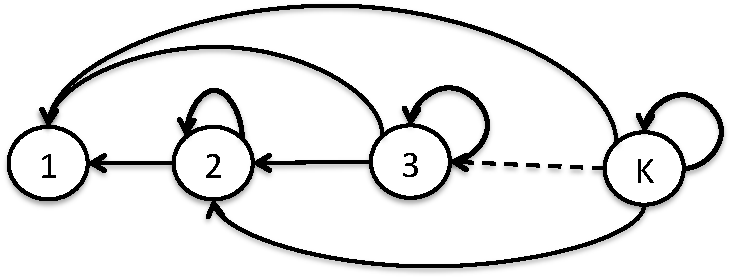
\includegraphics[scale=.4]{../Figures/SideInfoGraph.pdf}
	\caption{Side observation graph $G_S$}
	\label{fig:SideObservationGraph]}
\end{wrapfigure} 
In SAP with two sensors, only action $2$ provides partial information about the loss of both actions. In the case with $K>2$ sensors, by playing an action $k$, partial information about the loss from actions $l<k$ can be inferred by recursively applying the dominance property to each pair of sensors.  Further, any information provided by action $k>2$ is contained in that provided by all actions $k^\prime\geq k$ as $H_t(k) \subseteq H_t(k^\prime)$. 

This information structure can be represented by a directed graph $G_S=(V,E)$, where $|V|=K$ and $E=\{(i,j): 1<i\leq j\leq K \}$. Note that $G_S$ has self loops for all nodes except for node $1$. The nodes in $G_S$ represents actions of in SAP and an edge $(i,j)\in E$ implies that actions $i$ provides information about action $j$. The side-observation graph for the SAP is shown in Figure (\ref{fig:SideObservationGraph]}).

We now have all the ingredients to relate SAP problem with MAB.
\begin{thm}
	\label{thm:K-SAPRegret}
Let the dominance condition (\ref{eqn:DominanceCondition}) holds. Then SAP is regret equivalent to a MAB with side-observation graph $G_S$. 
\end{thm}
Then, from (\ref{eqn:MABLowerBound}), we immediately obtain following regret lower bound for SAP. 
\begin{proposition}[SAP regret lower bound]
	Let $\pi$ be any policy on SAP such that it pulls the suboptimal arm only sub polynomial many times, i.e., $\mathbb{E}[N^\psi_i(T)]=o(T^a)$ for all $a>0$ and $i\neq i^*$. Then,
	\begin{equation}
	\liminf_{T \rightarrow \infty} R^\psi_T(\pi)/\log T \geq \kappa \mbox{	where  }
	\end{equation}
		\begin{align}
	\kappa=&\displaystyle\min_{\{w_i\}}\sum_{i \in [K]}(\mu_{i^*}- \mu_i) w_i \nonumber\\
	& \mbox{subjected to} \sum_{j i}w_i\geq 1/D\left(\mu_i + \sum_{j<i} c_j \| \mu_{i^*} + \sum_{j<i^*} c_j \right ) \mbox{  for all } i\in [K]\\
	& w_i \geq 0 \mbox{ for all } i \in [K]. \nonumber
	\end{align}
\end{proposition}

\begin{proposition}[K-SAT regret upper bound]
Given a SA-problem $\psi$,	there exists a policy $\pi\in \Pi^\psi$ such that
\begin{equation}
	R^\psi_T(\pi)\leq \mathcal{O}(\log T) + \mathcal{O}(K^2). 	
\end{equation}
\end{proposition}
As discussed in the proof of Theorem \ref{thm:K-SAPRegret}, using  
 UCB-LP on side-observation graph $G_S$ we can obtain a policy for SAP that maintains regret guarantee of UCB-LP which is given as $\mathcal{O}(\xi(G_S)\log T) + \mathcal{O}(K^2)$. Now the claim follows by noting that $\xi(G_S)=1$. 



%
%\section{Extension to Multi-Stage and Multi-Action setting}
% 
% \subsection{Information and Side Observations:}
% on the feedback observed, we continue to assume that the dominance condition holds across the stages, i.e., for all $1\leq i\leq K-1$
% \begin{equation}
% \label{eqn:DominanceMultiStage}
%\mbox{ if } \hat{Y}_t^i=Y_t  \implies  \hat{Y}_t^j=Y_t \mbox{ for all } i<j\leq K
% \end{equation}
% Then, each time action $i>1$ is played, we get the same type of information about the loss incurred by an action pair  $(j,j-1)$ as in the SAP problem using the pair  $\{\hat{Y}_t^j,\hat{Y}_t^{j-1}\}$ for each $1<j<i$. Thus, playing action $i>1$ provides side observations about all the actions $j\leq ii$. We refer to this setting as Multi stage Sensor Acquisition Problem (MSAP). 
% 
% The side-observation structure in the MSAP problem can be represented by a directed graph $G=(\mathcal{V}, \mathcal{E})$ where $|\mathcal{V}|=K$ and $\mathcal{E}=\{(i,j) \in \mathcal{V}\times \mathcal{V}: i\geq j, i>1\}$. Here,  $(i,j)\in \mathcal{E}$ implies that selecting $i$ provides information about the prediction loss of action $j$. The side-observation graphs is depicted in Figure (\ref{fig:SideObservationGraph]}). Note that an edge $(i,j) \in \mathcal{E}$ only implies that playing action $i$ provides some information about the losses of actions $i\leq j$, but not their true losses. In the following we establish that regret of MSAP is equivalent to a stochastic $K$-armed bandit with the same side-observation structure.
%  \subsection{Regret Equivalence}
% \begin{thm}
% 	A MSAP $(K, \mathcal{A}, (\gamma_i,c_i)_{i\in [K]}, (L(i), F(i))_{i \in \mathcal{A}} )$ with $K>2$ is regret-equivalent to a stochastic bandit problem $(N, (\nu_i)_{i \in [N]})$ with $N=K$ and side observation structure give by $G$.
% \end{thm}	
%Consider a $K$-armed stochastic bandit problem where  reward distribution $\nu_k$ has mean $\gamma_1-\gamma_k + \sum_{j=2}^k c_j$ for all $1\leq k\leq K$, and the side-observation from arms is given by graphs $G$ . Given an arbitrary policy $\pi$ for the MSAP  that uses the side-information, we obtain a  policy BanditG($\pi$) for the bandit problem as follows: if BanditG($\pi$) played arm $i\neq 1$ in the previous round, it inputs the feedback observed from all arms $i\leq j$ to $\pi$ and copies $\pi$'s choice for next action. If BanditG($\pi$)  played arm $1$ in the previous round, it simply copies $\pi$'s choice for next action. Conversely, suppose $\theta$ is an arbitrary policy for the bandit problem with side-observation structure $G$, let MSAP($\theta$) denote a policy for MSAP that consults $\theta$ as follows: if MSAP($\theta$) played action $i$ in the previous round it inputs feedback vector $(0, \boldsymbol{1}_{\{\hat{Y}_t^j\neq \hat{Y}_t^{j-1} \}}, \forall \; j\leq 1)$ to $\theta$ and copies its choice for next action. Otherwise it simply copies $\theta$'s choice for next action.
%
%We next show that regret of BanditG($\pi$) on the bandit problem is same as that of $\pi$ on MSAP, 
% and regret of MSAP($\theta$) on MSAP is same as regret of $\theta$ on the bandit problem. 
% 
%For any strategy $\pi$, the expected regret of the MSAP can be expressed as 
%\begin{eqnarray}
%R_T(\pi) &=&\sum_{i=1}^{K}\left [ \left (\gamma_{i}+\sum_{j\leq i} c_j\right )-\left (\gamma_{i^*}+\sum_{j\leq i^*} c_j\right )\right ]\mathbb{E}[N_i(T)]\\
%&=&\sum_{i=1}^{K} \left[\left (\gamma_1+c_1-\gamma_{i^*}-\sum_{j\leq i^*} c_j \right )-\left (\gamma_1+c_1- \gamma_{i}-\sum_{j\leq i} c_j \right )\right ]\mathbb{E}[N_i(T)]
%\end{eqnarray} 
%where we added and subtracted $\gamma_1+c_1$ from each term. Now, notice that this is the expected regret of the policy on a stochastic bandit where the mean rewards  are 
%\begin{equation}
%\gamma_1+c_1 - \gamma_i - \sum_{j\leq i} c_j \quad \mbox{for } i=1,2,\cdots, K. 
%\end{equation}
%\begin{remark}
%Note that the some of mean 	values $\gamma_1+c_1 - \gamma_i - \sum_{j\leq i} c_j$ need not be positive. Since most of the stochastic bandit algorithms assume that reward lie in the interval $[0,1]$, they may not be directly applicable to our setting. However, this can be over come by setting the distributions of arm $k$, $\nu_k$, to have mean $\gamma_1+c_1 - \gamma_i - \sum_{j\leq i} c_j + \sum_{k=2}^K c_k$. Note that we translated the mean of each arm by the same amount this does not change the regret value. For $k=2$, this recovers the SAT problem and Theorem \ref{thm:SATRegret} holds
%\end{remark}
%$\wedge$
%
%\begin{thm}[Upper Bound]
%	
%\end{thm}
%\begin{thm}
%	
%\end{thm}
%When we pull an arm  $i$, we observe a realization of a distribution with mean $\gamma_1 -\gamma_i$, but since the cost values are fixed, this is equivalent to observe realization of a distribution with mean $\gamma_1 +c_1-\gamma_i + \sum_{j\leq i}c_i$. Thus, the sensor selection problem with mean costs $\{\gamma_i + \sum_{j\leq i}c_i\}$ is equivalent to a stochastic multi-armed problem with mean rewards $\{\gamma_1+c_1 -\gamma_i - \sum_{j\leq i}c_i\}$. 

% \alglanguage{pseudocode}
% \begin{algorithm}[!h]
% 	\footnotesize
% 	\caption{StAT-K}
% 	\label{Algorithm:Stochastic Apple Tasting1}
% 	\begin{algorithmic}[1]
% 		\State \textbf{Input:}
% 		\State $c_k$ cost of sensor $k=2\cdots,K $
% 		\State \textbf{Initialization:}
% 		\State Play $a_K$ once, observe $X_{j,t}^i$, for all $K \geq j>i\geq 1$
% 		\State $N_{K}(1)\leftarrow 1 $, $Y_{j,1}^i\leftarrow X_{j,1}^i$ and $\hat{\mu}_{j,1}^i\leftarrow \frac{Y_{j,1}^i}{N_{K}(1)}$ for all $K \geq j > i\geq 1$
% 		\For {$t = 2,3\cdots$}
% 		\State {\bf Select the best action optimistically. How? We can use pairwise information to select the best action as follows}  
% 		\For {$j=2,3,\cdots, K$}
% 		\State $I\leftarrow 1$
% 		\If {$\hat{\mu}_{j,t-1}^I + \sqrt{\frac{6\log t}{\sum_{k\geq j} N_{k}(t-1)}} > \displaystyle \sum_{k=I+1}^{j}c_k$}  \quad //Checks if action $I$ is better than action $i$,
% 		\State $I\leftarrow j$
% 		\Else
% 		\State $I \leftarrow I$
% 		\EndIf
% 		\EndFor
% 			\State play action $a_I$ and observe $X_{I,t}^i$ for all $I>i\geq 1$,
% 			\State $N_{I}(t) \leftarrow N_{I}(t-1)+1$, $Y_{I,t}^i\leftarrow Y_{I,t-1}^j+X_{I,t}^i$ for all $ I>i \geq 1$
% 			\State $\hat{\mu}_{I,t}^i \leftarrow \frac{Y_{I,t}^i}{\sum_{k=I}^{K}N_k(t)}$ for all $ I>i \geq 1$
% 		\EndFor 
% 		
% 		\Statex
% 	\end{algorithmic}
% 	% \vspace{-0.4cm}%
% \end{algorithm}
% 
%
%\section{Algorithm}
%Let $X_{j,t}^i=\boldsymbol{1}_{\{\hat{y}^{i}_t \neq \hat{y}^j_t\}}, j>i$ denote whether the predictions of sensors $i$ and $j$ agree or not in round $t$. Note that $X_{j,t}^i$ is observed whenever learner selects action $a_k, k>j$. Let $\hat{\mu}_{j,t}^i$ denote the empirical mean of the samples $\{X_{j,t}^t\}$ observed till time $s$, given by
%\begin{equation}
%\hat{\mu}_{j,s}^i= \frac{\sum_{t=1}^s X_{j,t}^i\boldsymbol{1}_{\{I_t\geq j\}}}{\sum_{k=j}^{K}N_k(s)}.
%\end{equation}
%
%
%{\bf Remarks: We discussed the strategy in Algorithm-1 (StAT-K). Consider the case of perfect knowledge of $\gamma_i$'s and assume $j^{th}$ action is optimal. Then we know that $\gamma_i - \gamma_j> \sum_{k=i+1}^{j} c_k$ for all $i<j$ and $\gamma_j - \gamma_i < \sum_{k=j+1}^{i} c_k$ for $j<i$. However, after estimating the $\gamma_i$'s and selecting the best action optimistically as in StAT-K does not lead to similar argument, i.e.,  suppose in round $t$, $I^{th}$ action is selected by StAT-K, then the following need not hold.}
%
%\[{\hat{\mu}_{I,t-1}^j + \sqrt{\frac{6\log t}{\sum_{k\geq I} N_{k}(t-1)}} > \displaystyle \sum_{k=j}^{I}c_k} \quad for \;\;  I>j\]
%and
%
%\[{\hat{\mu}_{j,t-1}^I + \sqrt{\frac{6\log t}{\sum_{k\geq j} N_{k}(t-1)}} < \displaystyle \sum_{k=I+1}^{j}c_k} \quad for \;\; j> I\]
%

